%Git-rapport
\documentclass[a4paper]{article}

\usepackage[swedish]{babel}
\usepackage[utf8]{inputenc}
\usepackage{graphicx}
\setcounter{secnumdepth}{4}
\usepackage{titlesec}
\usepackage{caption}
\usepackage{float}
%For figures
\graphicspath{ {Figures/} }
\captionsetup{justification=centering}

\begin{document}

\begin{titlepage}
\centering
{\bfseries\huge Projektrapport DAT290}

\vspace{10mm}

{\Large Radiostyrd Bil, Grupp 07}

\vspace{20mm}

{\Large \itshape{Anders Berggren Sjöblom, Johanna Gudmandsen, Gustav Holst, Joakim Junttila, Henrik Klein Moberg, Carl Lundgren, Stanisław Zwierzchowski}}

\vspace{10mm}

%Vet ej vilket datum som ska stå
{2016-10-23}


\normalsize{
\begin{table}[b]
\centering
\begin{tabular}{|l|l|l|}  \hline
         & \bf Namn & \bf Datum   \\ \hline \hline
Granskad & NAMN     & DATUM        \\ \hline
Godkänd  & NAMN     & DATUM         \\ \hline
\end{tabular} 
\end{table}}
\end{titlepage}

\tableofcontents

\newpage
\noindent {\Large \bf Ordlista}
\\\\
{\bf ADC} - Analog to digital converter, översätter analoga värden i enheten Volt till digitala värden~\cite{ADC}.
\\\\
{\bf Android} - Ett operativsystem~\cite{Android}.
\\\\
{\bf ARM} - En processorarkitektur~\cite{chalmersARM}.
\\\\
{\bf AT-kommando} - En instruktion som används för att kontrollera modem~\cite{AT}.
\\\\
{\bf Avståndsmätare} - Mäter avstånd från ett objekt med hjälp av ultraljud och dess eko~\cite{DistMeasure}. Modul som används i detta projekt är HC-SR04.
\\\\
{\bf Bluetooth-moduler} - Är antingen sändare eller mottagare och möjliggör för radiofrekvensiell överföring genom parning mellan moduler~\cite{Bluetooth}. Modul som används i detta projekt är HC-05.
\\\\
{\bf GPIO} - General-purpose input/output~\cite{chalmersARM}.
\\\\
{\bf Oscilloskop} - Instrument som används till att mäta elektriska signaler under en viss tid~\cite{oscilloscope}.
\\\\
{\bf Potentiometer} - En elektrisk komponent som med hjälp av ett variabelt motstånd kan begränsa spänning~\cite{Potentiometer}.
\\\\
{\bf PWM-signaler} - PWM eller Pulse Width Modulation är en moduleringsteknik som mest används för att styra mängden elektrisk ström som förs till exempelvis en motor~\cite{PWM}.
\\\\
{\bf RF-moduler} - Radiofrekvensmoduler. Är antingen sändare eller mottagare och möjliggör för radiofrekvensiell överföring~\cite{RFModule}.


\newpage
\section{Introduktion}
Radiostyrda bilar började produceras på mitten av 60-talet~\cite{RCHistory}. Dessa drevs då med hjälp av bensin och körde relativt långsamt. Ett drygt decennium senare ersattes motorerna med elektriska varianter och kort därefter började tävlingar anordnas. Detta ledde till en väldig popularitet för radiobilen som hobby och utvecklingen kom då att fokusera på konstruktion av bilar som kunde uppnå högre hastigheter. Trots dessa mindre förändringar har den radiostyrda bilens uppbyggnad i det stora hela förblivit densamma.

\subsection{Syfte}

Syftet med detta projekt är att uppdatera den klassiska radiostyrda bilen genom att ersätta befintlig sändare samt mottagare i en radiostyrd bil med nya datorer och även möjliggöra styrning från en telefonapplikation. Avsikten är även att implementera en kontrollapplikation som ska kunna stoppa bilen från att kollidera. Följden av detta blir en produkt mer anpassad till aktuell teknik och det erhålls på så sätt en mer modern teknisk produkt.


\subsection{Mål}
Projektets övergripande syfte bryts upp i delmål som är angivna nedan.

\begin{itemize}
\item Den befintliga sändaren samt mottagaren som finns i handkontrollen respektive bilens elektronik byts ut mot ARM-baserade system, datorenheten MD407 (se Figur 1). Dessa kontrolleras vid färdig produkt via Bluetooth.
\item En kontrollapplikation implementeras. Bilen ska kunna köra rakt fram och på ett avstånd av 1 cm från ett hinder självständigt bromsa in utan att kollidera.
\item Utveckling av Androidapplikation som möjliggör att bilen kan manövreras trådlöst genom en Androidtelefon via Bluetooth.
\end{itemize}

\begin{figure}[H]
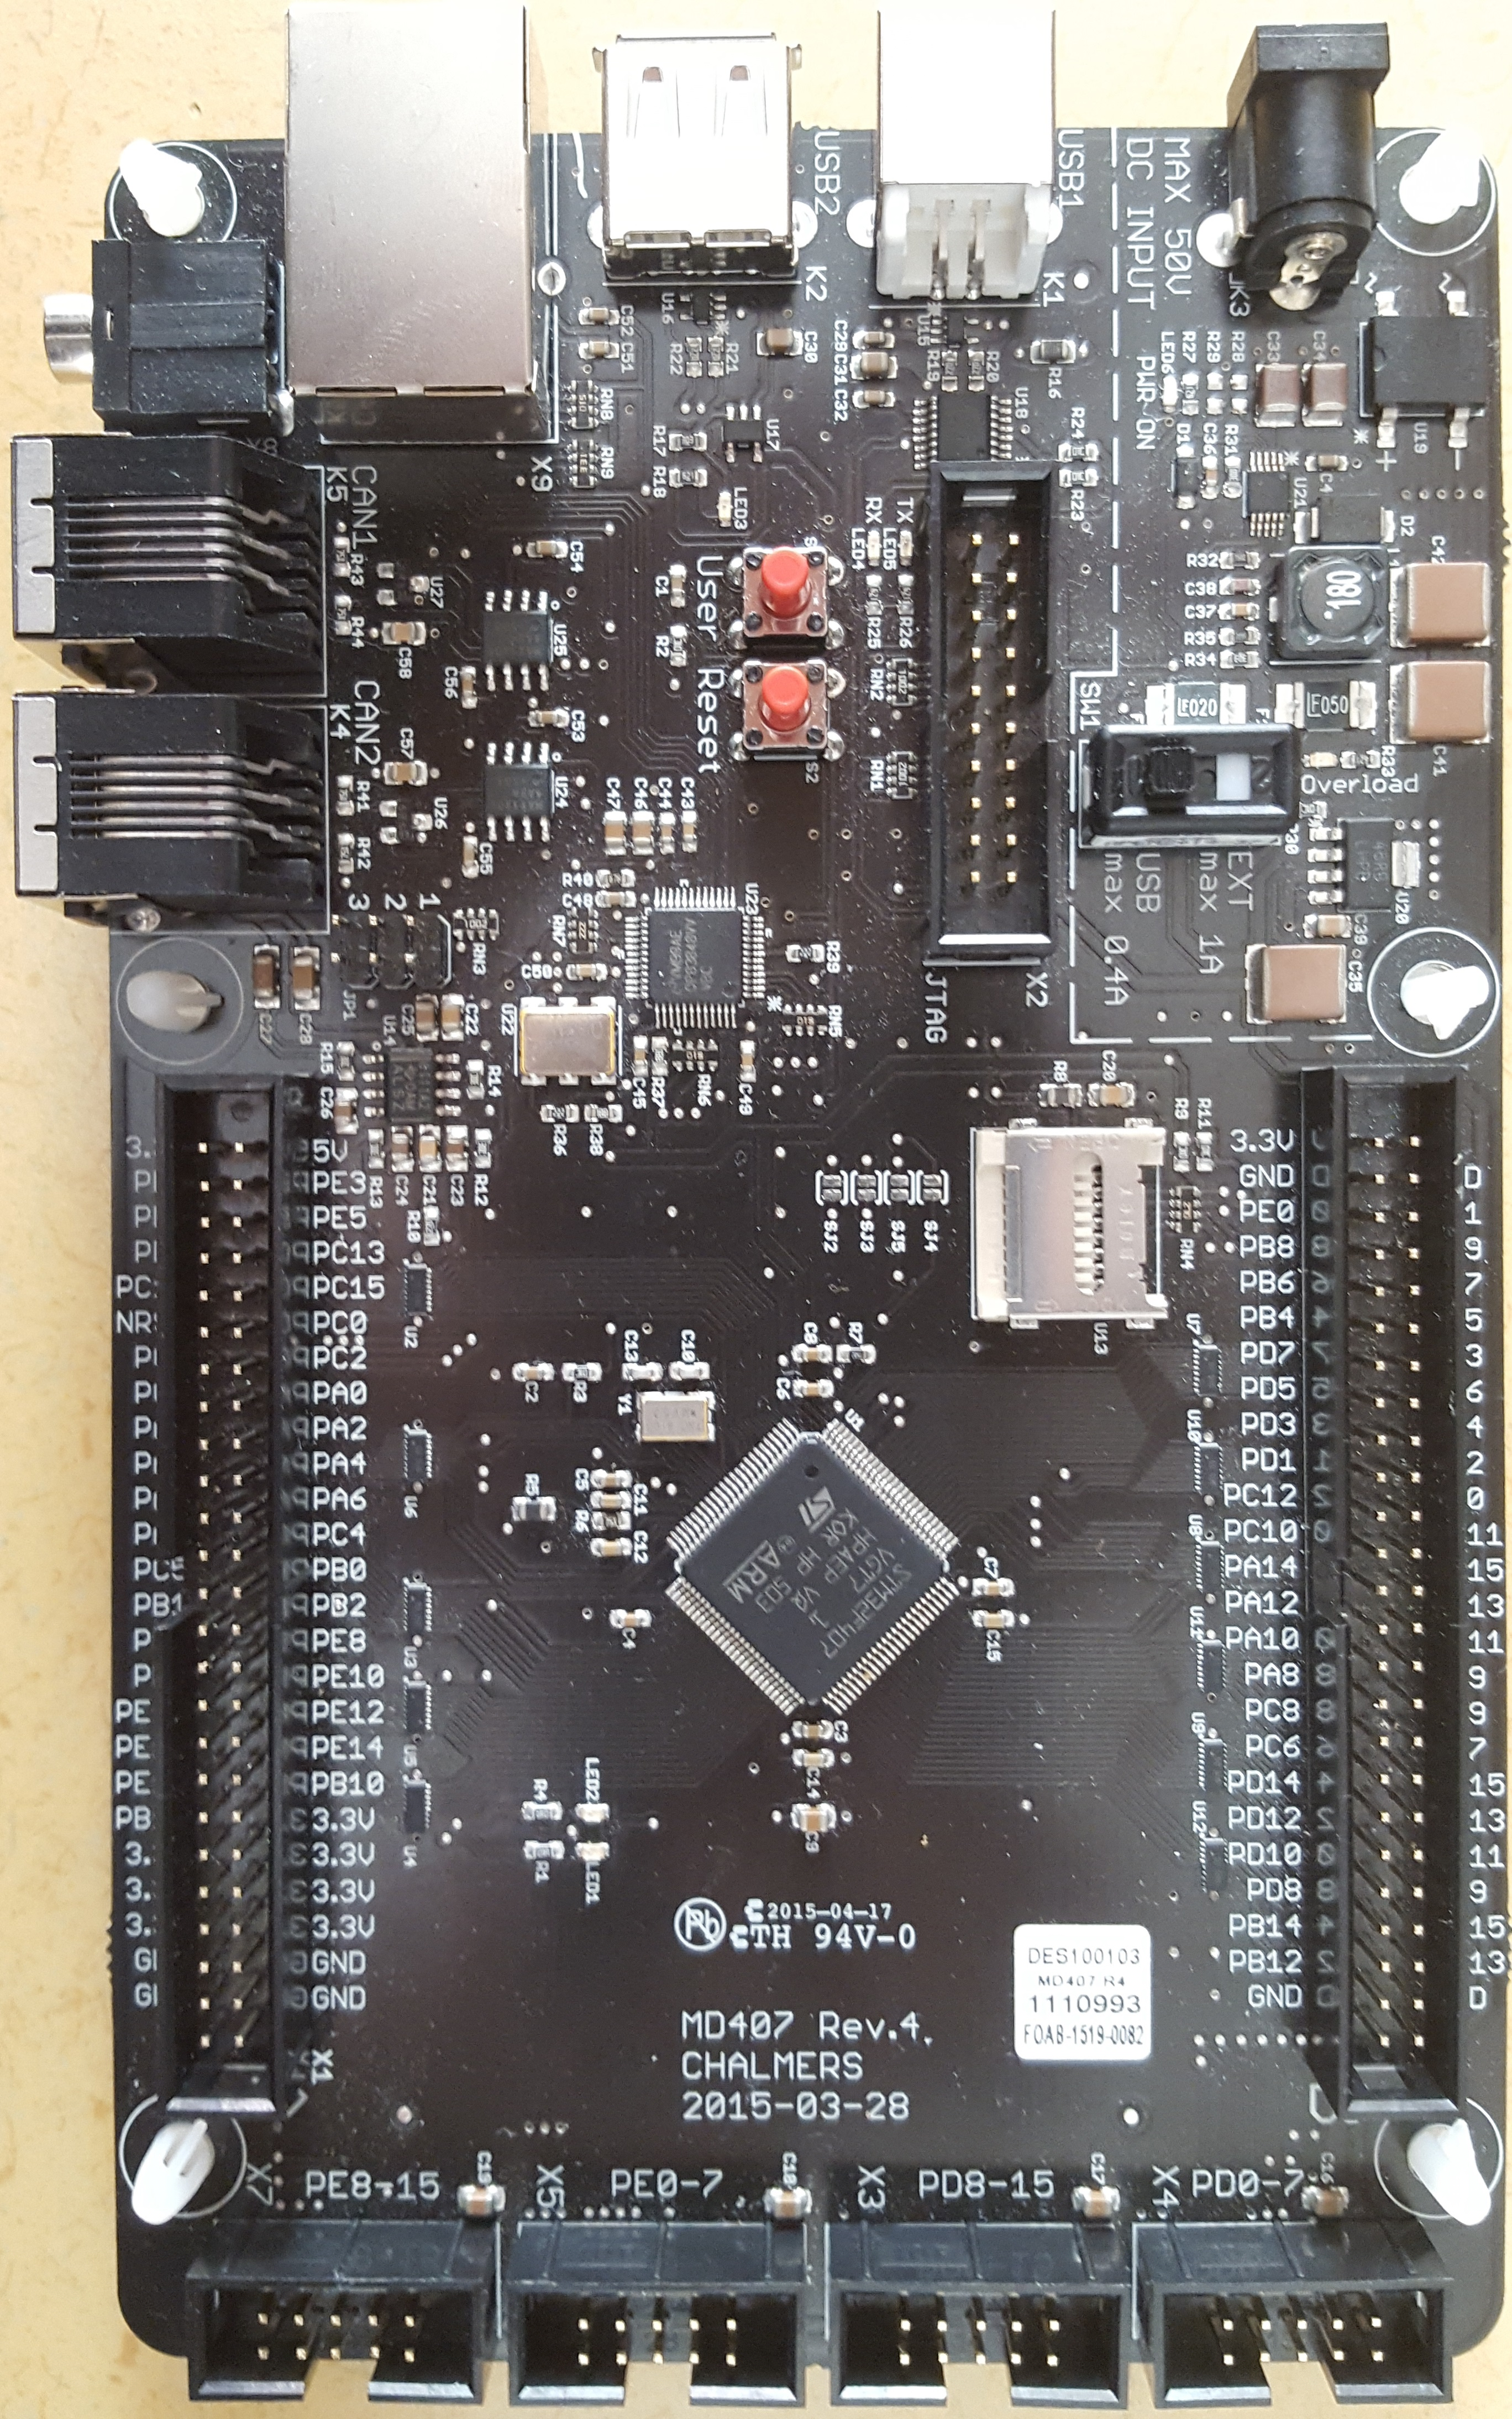
\includegraphics[scale=0.03]{MD407.jpg} \hspace{2mm}
\centering
\caption{\it MD407, en ARM-dator.}
\end{figure} 

\subsection{Arbetsmetod}
I detta avsnitt finns en överblick av hur projektet utförts vid olika moment. Det börjar med två avsnitt över projektets generella specifikationer och följs av en beskrivning av varje komponent som konstrueras i systemet. Dessa är angivna i ordningen de utförs.

\subsubsection{Projektledning}
Dokumentation och kommunikation utförs enligt planen för projektet. Ett versionshanteringssystem, Git, används för att enkelt kunna lagra filer mellan olika datorer. Applikationen Slack utnyttjas för att möjliggöra strukturerad kommunikation och utöver detta sker möten en gång i veckan för att varje projektgruppsmedlem ska få aktuell information. Veckovisa meddelanden för projektets fortskridande har givits till uppdragsgivaren. Detta på grund av att det ska vara enkelt att följa utvecklingen. Under projektets gång delades gruppen upp i mindre arbetslag som självständigt fokuserade på första och andra målet, tredje målet samt dokumentationen. Detta gjordes för att kunna arbeta parallellt med uppgifter och således få mer djupgående förståelse för dessa.

\subsubsection{Kodning}
Standarder för kodning är bestämda för underlätta implementation. Programkoder är för samtliga komponenter förutom Androidapplikationen skrivna i C med utvecklingsmiljön Codelite. För att kunna överföra kod till datorenheterna som ersätter mottagare och sändare utnyttjas programmet ETERM. En kompilerad kod laddas då upp via en direktkoppling mellan datorn där koden skrivs och respektive enhet. Programmet kan därefter exekveras. Hjälpfunktioner till all programkod har erhållits av uppdragsgivarens samt STMicroelectronics~\cite{STM} kodbibliotek. Utvecklingen av Androidapplikationen skedde istället i Java och importerades sedan till Android Studio, en miljö där stöd för att skapa Androidapplikationer finns.

\subsubsection{Styrsignaler}
Projektet inleds med att mäta upp befintliga styrsignaler. För att kunna återskapa signalerna som skickas från den ursprungliga mottagaren till bilens styrelektronik mättes signalerna upp med hjälp av ett oscilloskop. Det som möjliggjorde detta var ett tillhandahållet kretskort som kopplat till bilens kontrollenhet separerar signalerna. Bilens samtliga funktioner testades och utslagen blev de värden som användes till verifiering för replikering av identiska styrsignaler. Signalerna är av typen PWM och både dess cykeltid och frekvens mättes upp i motorns och rattutslagens maximala lägen. 


\subsubsection{Konstruktion av mottagare}
Den nya mottagaren återskapar PWM-signaler identiska till det ursprungliga systemet. En MD407 ersätter den ursprungliga mottagaren och dess systemklocka utnyttjas för att skicka rätt styrsignaler till korrekt styrelektronik. Dessa värden verifieras med oscilloskop samt på hårdvaran för att kunna säkerställa att de replikerande styrsignalerna är identiska i jämförelse med de ursprungliga. 





\subsubsection{Konstruktion av sändare}
En MD407 ersätter sändaren. Reglage för styrning implementeras med hjälp av två potentiometrar (se Figur 2) som kopplas till datorenheten. Dess värden kan då enkelt erhållas av MD407 som sedan översätter dessa analoga värden till digitala via en integrerad ADC. Detta implementeras med hjälp av stödfunktioner från de tidigare nämnda kodbiblioteken.

\begin{figure}[H]
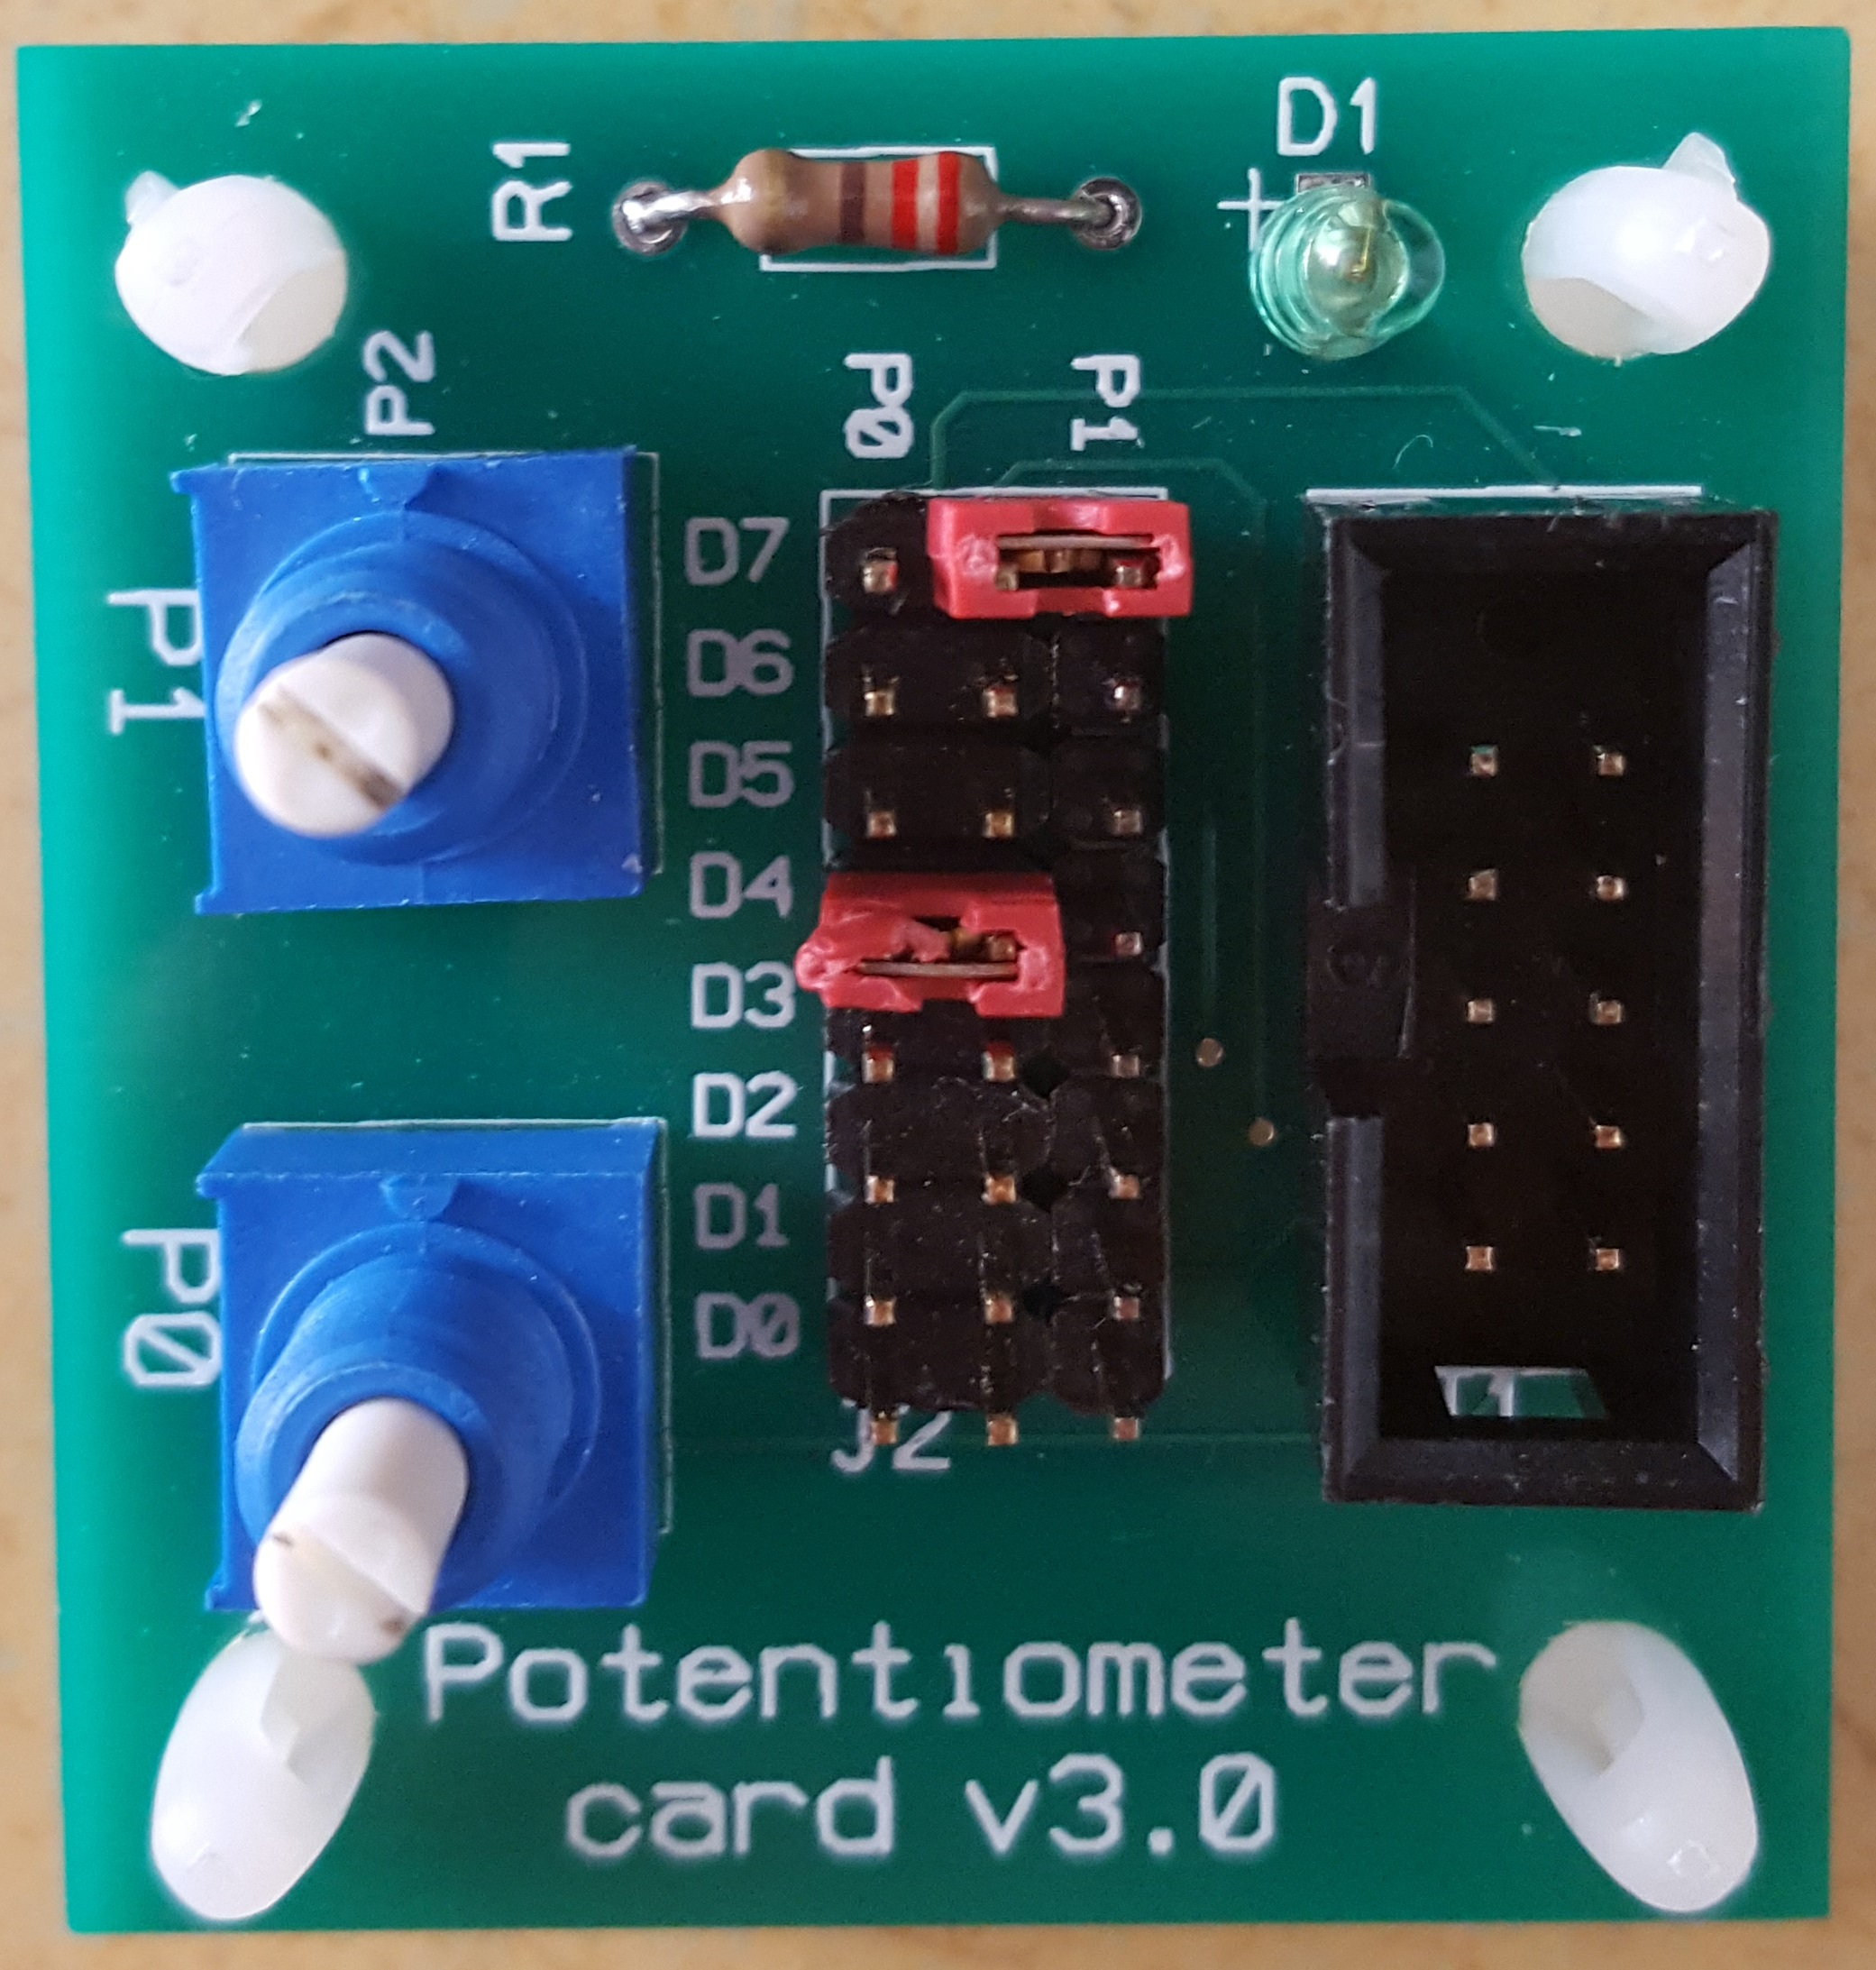
\includegraphics[scale=0.04]{Potentiometer.jpg}
\centering
\caption{\it En potentiometer.}
\end{figure} 

\subsubsection{Radiolänk mellan mottagare och sändare}
Datorenheterna kommunicerar via en radiolänk. Primärt kopplas en RF-mottagare och -sändare (se Figur 3) till respektive enhet för att möjliggöra ett informationsflöde över 433MHz-bandet. När systemet fungerar med dessa ersätts de av Bluetooth-moduler (se Figur 3) som istället kommunicerar över en frekvens av 2.4GHz. Kommunikation över Bluetooth kräver initiering av roller till modulerna vilket görs genom AT-kommandon. 



\begin{figure}[H]
\centering
\includegraphics[scale=0.048]{RF-transmitter.jpg}
\includegraphics[scale=0.04]{RF-receiver.jpg} \\ \vspace{2mm}
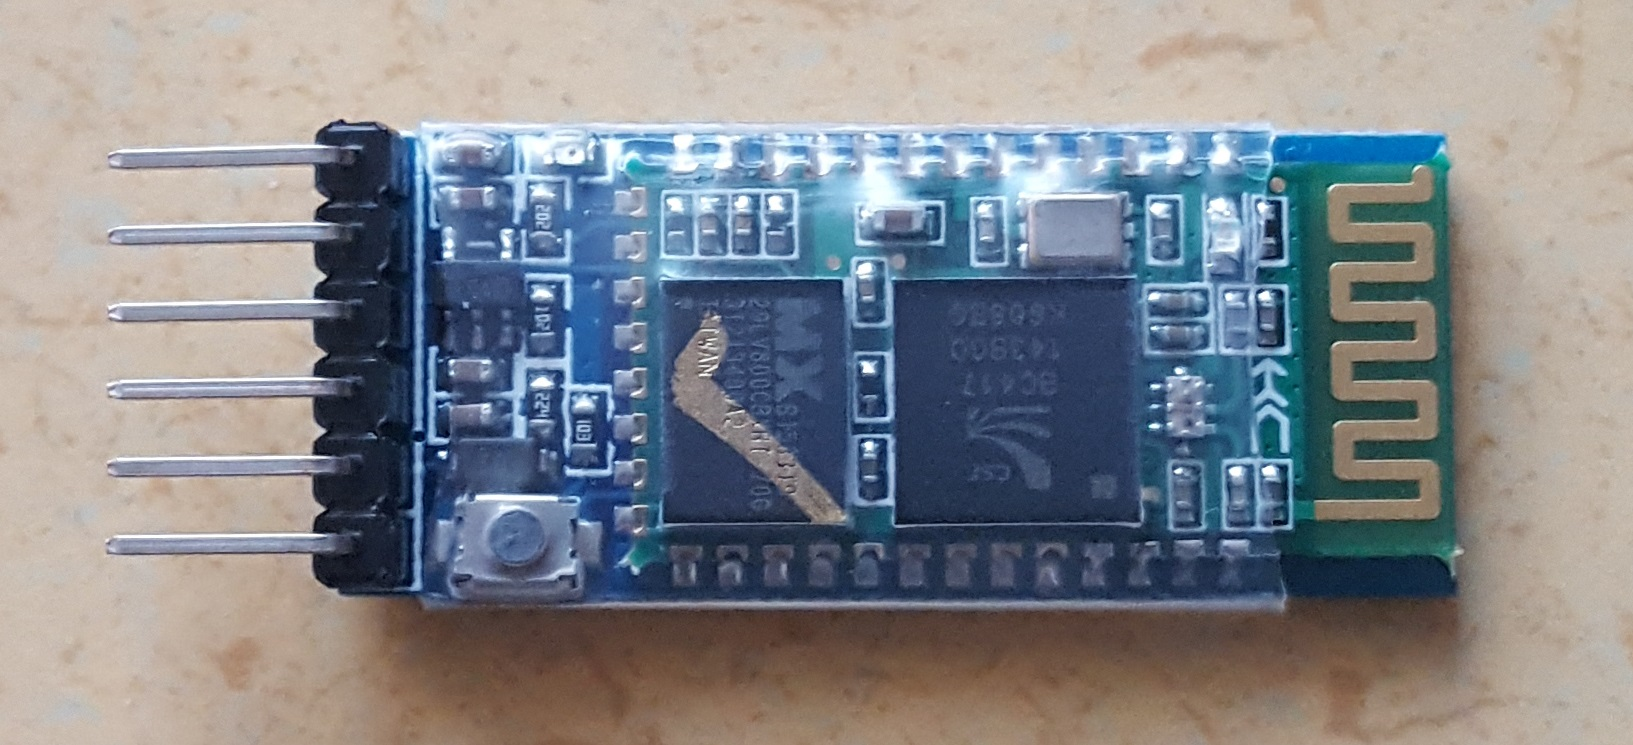
\includegraphics[scale=0.06]{BluetoothFront.jpg}
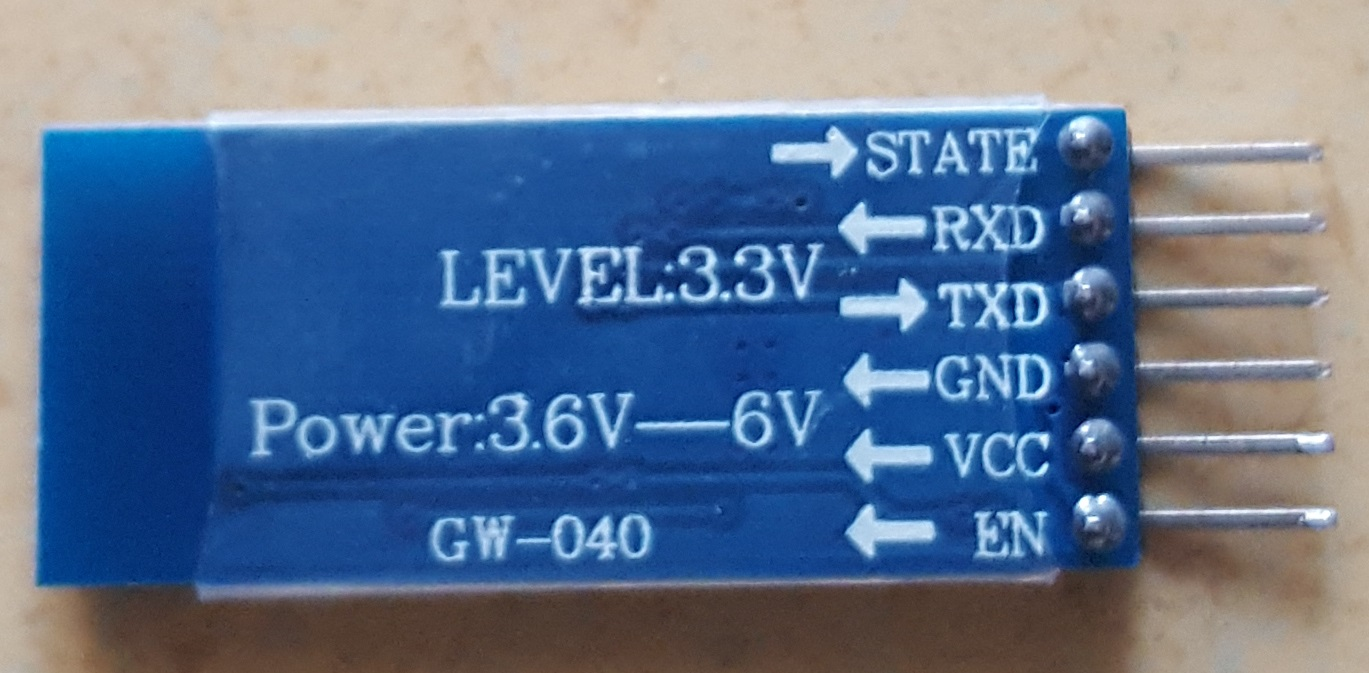
\includegraphics[scale=0.066]{BluetoothBack.jpg}
\caption{\it På övre raden ses en RF-mottagare samt RF-sändare (i angiven ordning) och på undre raden en Bluetooth-moduls framsida samt baksida (i angiven ordning)}
\end{figure} 

\vspace{5mm} \noindent
Radiolänken verifieras kontinuerligt. Mottagar- och sändarmodul kopplas in vid varje tillfälle under hela verifikationstiden för att erhålla det konstanta flödet av testning. Utöver detta används ett oscilloskop för att kunna säkerställa hur kommunikationen mellan mottagar- och sändarmodul fungerar. Det kopplas då till sändaren respektive mottagaren för att verifiera att ett värde i sändarnoden motsvarar korrekt värde i mottagarnoden. Vid tillfällen då felsökning genomförts på grund av felaktiga signaler till mottagarmodulen har enheterna direktkopplats via en kabel för att kunna utesluta radiolänken som problem.


\subsubsection{Konstruktion av Androidapplikation}
Mobilapplikationen följer ett antal specifikationer. Den ska vara funktionell på en Androidtelefon och kopplas till den radiostyrda bilen via Bluetooth. Dess styrning implementeras genom reglage på skärmen som enkelt kan dras åt olika håll. Denna utökning av systemet verifieras genom samtliga funktioner samt att applikationens reglage ger rätt respons hos bilens styrelektronik. 


\subsubsection{Konstruktion av kontrollapplikation}
Kontrollapplikationen implementeras i mottagaren. Aktivering av denna applikation möjliggörs i båda sändarnoderna. Den ska kunna undvika kollision och detta möjliggörs med en avståndsmätare (se Figur 4) fastkopplad på bilen. Denna aktiveras med hjälp av fördröjningsfunktioner från de tillhandahållna biblioteken. Komponenten skickar sedan data till mottagaren som specificerar avståndet till närmsta hinder. Utdatan från avståndsmätaren mäts även upp med hjälp av oscilloskop för att säkerställa att kontrollapplikationen reagerar på rätt sätt vid olika värden. Dessa värden fångas upp av en funktion. Funktionen konstrueras och kalibreras för att utföra givet mål, att bromsa in helt innan ett hinder. Kalibrering sker via testning av funktionen med olika inställningar där effektiviteten utvärderas. 


\begin{figure}[H]
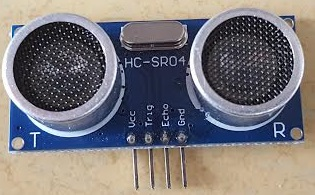
\includegraphics[scale=0.6]{DistanceMeasurementFront.jpg}
\centering
\caption{\it HC-SR04, avståndsmätaren i detta projekt.}
\end{figure} 



\newpage
\section{Teknisk beskrivning}
I denna sektion förklaras den tekniska delen av projektet. En bakgrund beskriver hur systemet fungerade ursprungligen. Detta följs av en översiktlig text över det ersättande systemet samt en sektion med mer detaljerande beskrivning över de separata delsystemen.


\subsection{Teknisk bakgrund}
För att kunna kontrollera en radiobil används en RF-sändare och en RF-mottagare ~\cite{RCTechnique}. Radiosignaler skickas från RF-sändaren och avkodas av RF-mottagaren i radiobilen, de kommunicerar över 2.4GHz-bandet. Dessa omvandlas då till elektroniska signaler som antingen kontrollerar bilens hastighet eller riktning. Parallellt med detta styrs även bilens hastighet, framåt eller bakåt, av motorns kraftutslag, medan riktningen beror på hjulens gradförskjutning. Bilens styrenhet omvandlar radiosignaler som sedan kontrollerar bilens rörelse.

\subsubsection{Styrsignaler}
Bilens styrsignaler kontrolleras av en kontrollenhet, MRX-242~\cite{projektDir}. Enheten fungerar simultant som radiomottagare och styrsignalsgenerator. I mening att replikera dessa finns även tillgång till ett ytterligare kopplingsblock.


\subsection{Systemöversikt}
Systemet har två huvuddelar, en MD407 samt en Androidapplikation som båda kan agera som sändarnod, och en MD407 som genererar signaler till motorerna.

\subsubsection{Styrning från MD407 till MD407}
\begin{figure}[H]
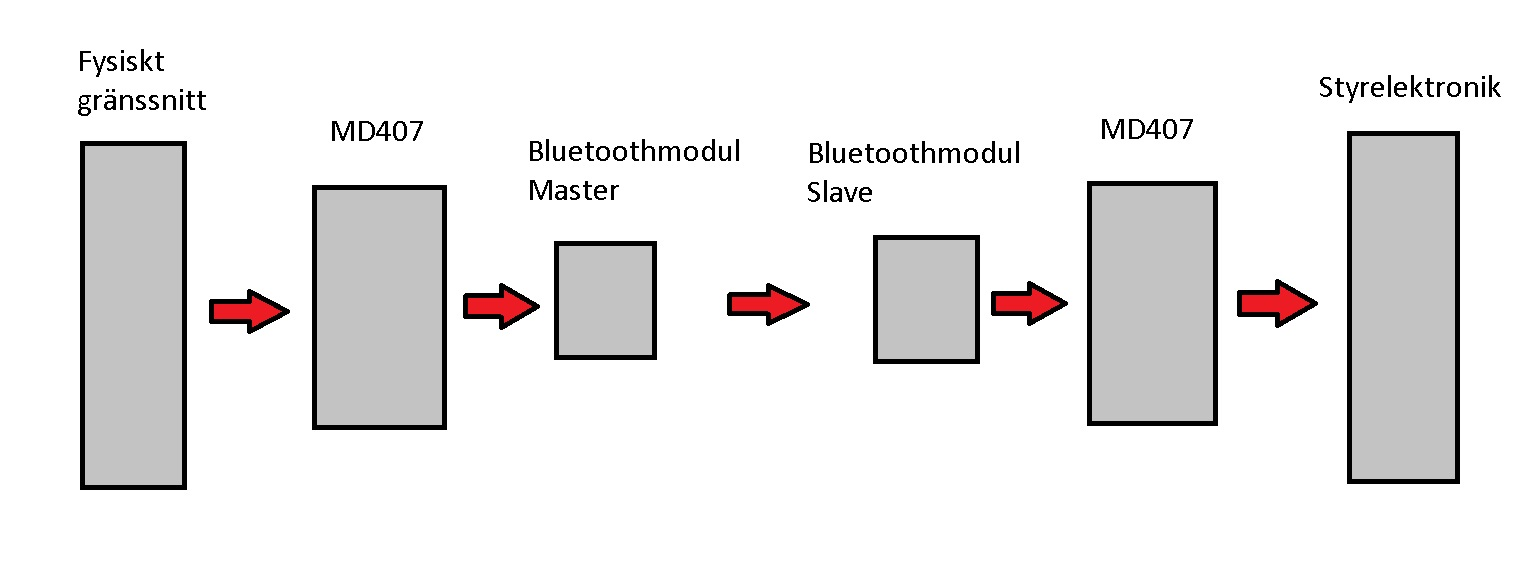
\includegraphics[width=\textwidth]{systemoversikt.jpg}
\centering
\caption{\it En översikt över systemet i blockformat med MD407 till MD407. Pilarna indikerar flödet av information, analogt eller digitalt.}
\end{figure} 


Enligt Figur 5 erhålls en överblick över hur systemet fungerar. Den sändande datorenheten MD407 får information från ett fysiskt gränssnitt, två potentiometrar, och skickar dessa värden via Bluetooth till den mottagande MD407 som tar emot värdena och överlämnar dessa till bilens styrelektronik som agerar efter dem.

\subsubsection{Styrning från Androidapplikation till MD407}
\begin{figure}[H]
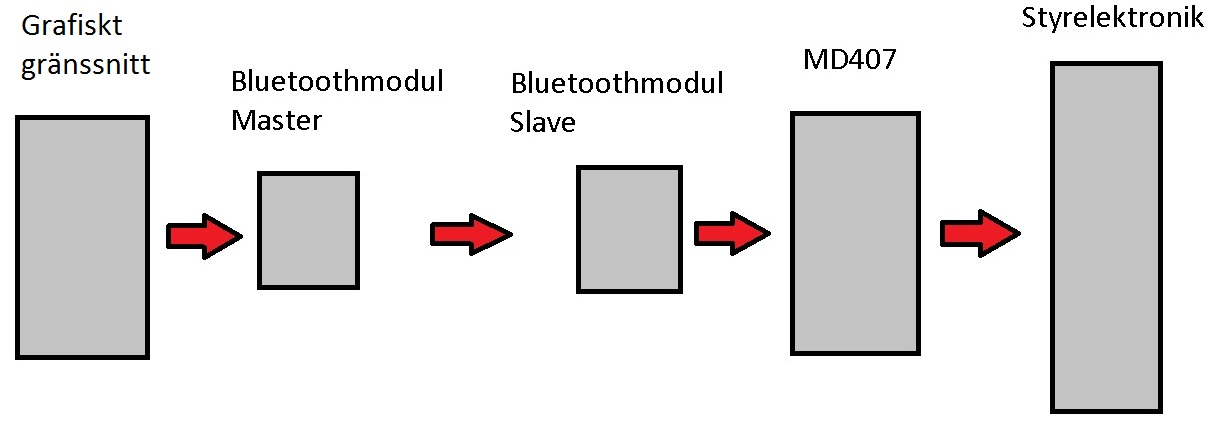
\includegraphics[width=\textwidth]{systemoversiktAndroid.jpg}
\centering
\caption{\it En översikt över systemet i blockformat med Androidapplikation till MD407. Pilarna indikerar flödet av information, analogt eller digitalt.}
\end{figure} 

Figur 6 visar en sammanfattning över systemet med en applikation som sändare. Observera att skillnaden mellan den tidigare styrningen är att Androidapplikationen skickar data genom telefonens integrerade Bluetooth-modul till mottagarens inkopplade. På samma sätt som tidigare analyseras sedan värdena och skickas till elektroniken i bilen.


\subsection{Delsystem}
Denna del av texten beskriver detaljerat hur de separata systemen fungerar. Ordningen baseras på flödet av information från sändare till mottagare och fram till bilens styrelektronik.




\subsubsection{MD407 som sändarnod}
Den sändande MD407 skickar värden från potentiometrarna till den mottagande enheten. Sändaren försörjer dess inkopplade potentiometrar med ström och läser konstant av utmatningsportarna för dess vridkontakter. På datorenheten finns en integrerad ADC, vilken tar emot värdena från potentiometrarna och översätter dessa från analoga till digitala värden. Det skickas sedan 8-bitars värden mellan sändare och mottagare vilka ställs in enligt specifikationerna i Figur 7. Ändras exempelvis vridkontakten på potentiometern för motorn ska kommandot initieras till det värde där mottagaren i sin tur sänder informationen till motorns elektronik. De 6 minst signifikanta bitarna beror på värdet datorenheten erhåller från potentiometrarna och tillsammans med kommandot skickas det seriellt från sändarens Bluetooth-modul och avläses i mottagarens.


\begin{figure}[H]
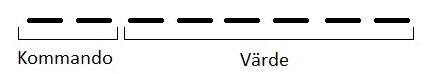
\includegraphics[scale=1]{aByteComVal.jpg}
\centering
\caption{\it Specifikationer av en byte som ständigt skickas seriellt skickas från sändare till mottagare.}
\end{figure} 


\subsubsection{Androidapplikation som sändarnod}
Androidapplikationen agerar som sändarnod. Denna ansluter först till mottagarens Bluetooth-modul för att möjliggöra kommunikation mellan dessa. På skärmen finns sedan virtuella reglage (se Figur 8) som emulerar ordinarie handkontrollens analoga funktion så att exempelvis hastighetsövergången är så jämn som möjligt. Applikationen har även en tilläggsknapp som aktiverar kontrollapplikationen. Via Bluetooth-anslutning skickas sedan bytes seriellt från telefonen till mottagarens Bluetooth-modul. Detta följer likadant protokoll som tidigare nämnts där de 2 mest signifikanta bitarna i varje byte bestämmer vilken sorts signal som ska ändras och de resterande bitarna bestämmer med vilket värde detta ska ske. 

\begin{figure}[H]
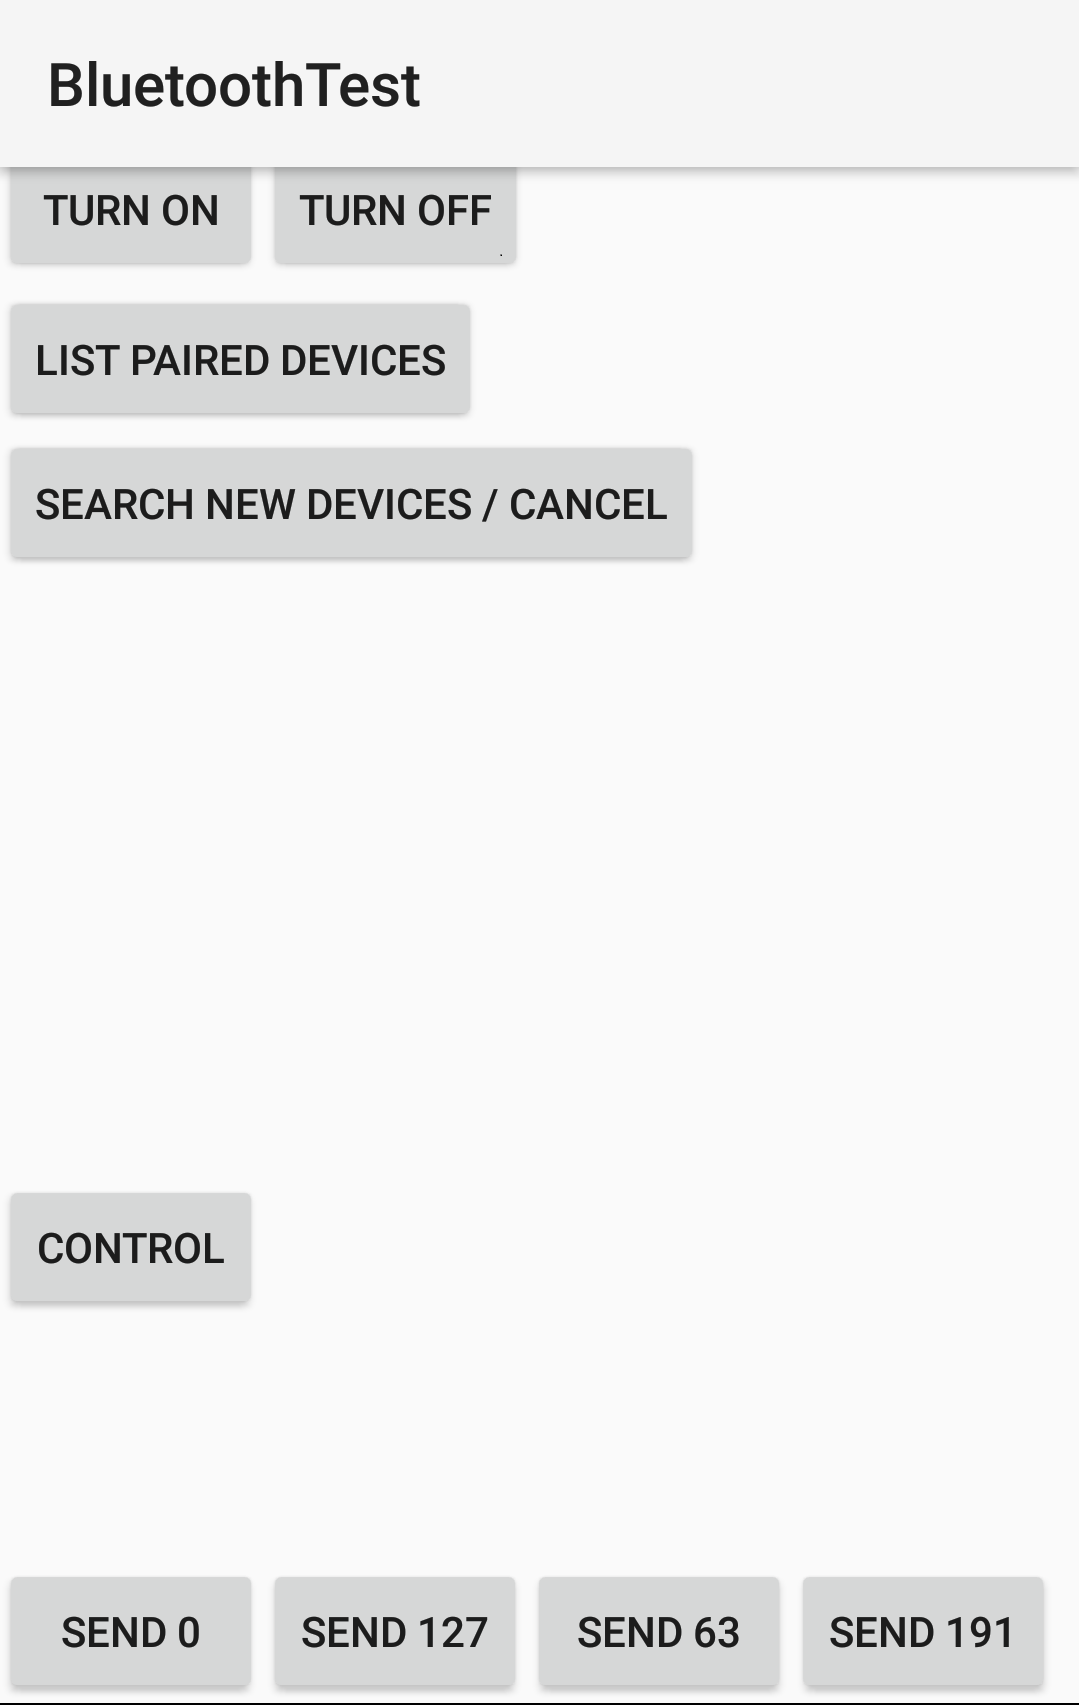
\includegraphics[scale=0.2]{Mobilapp1.png}
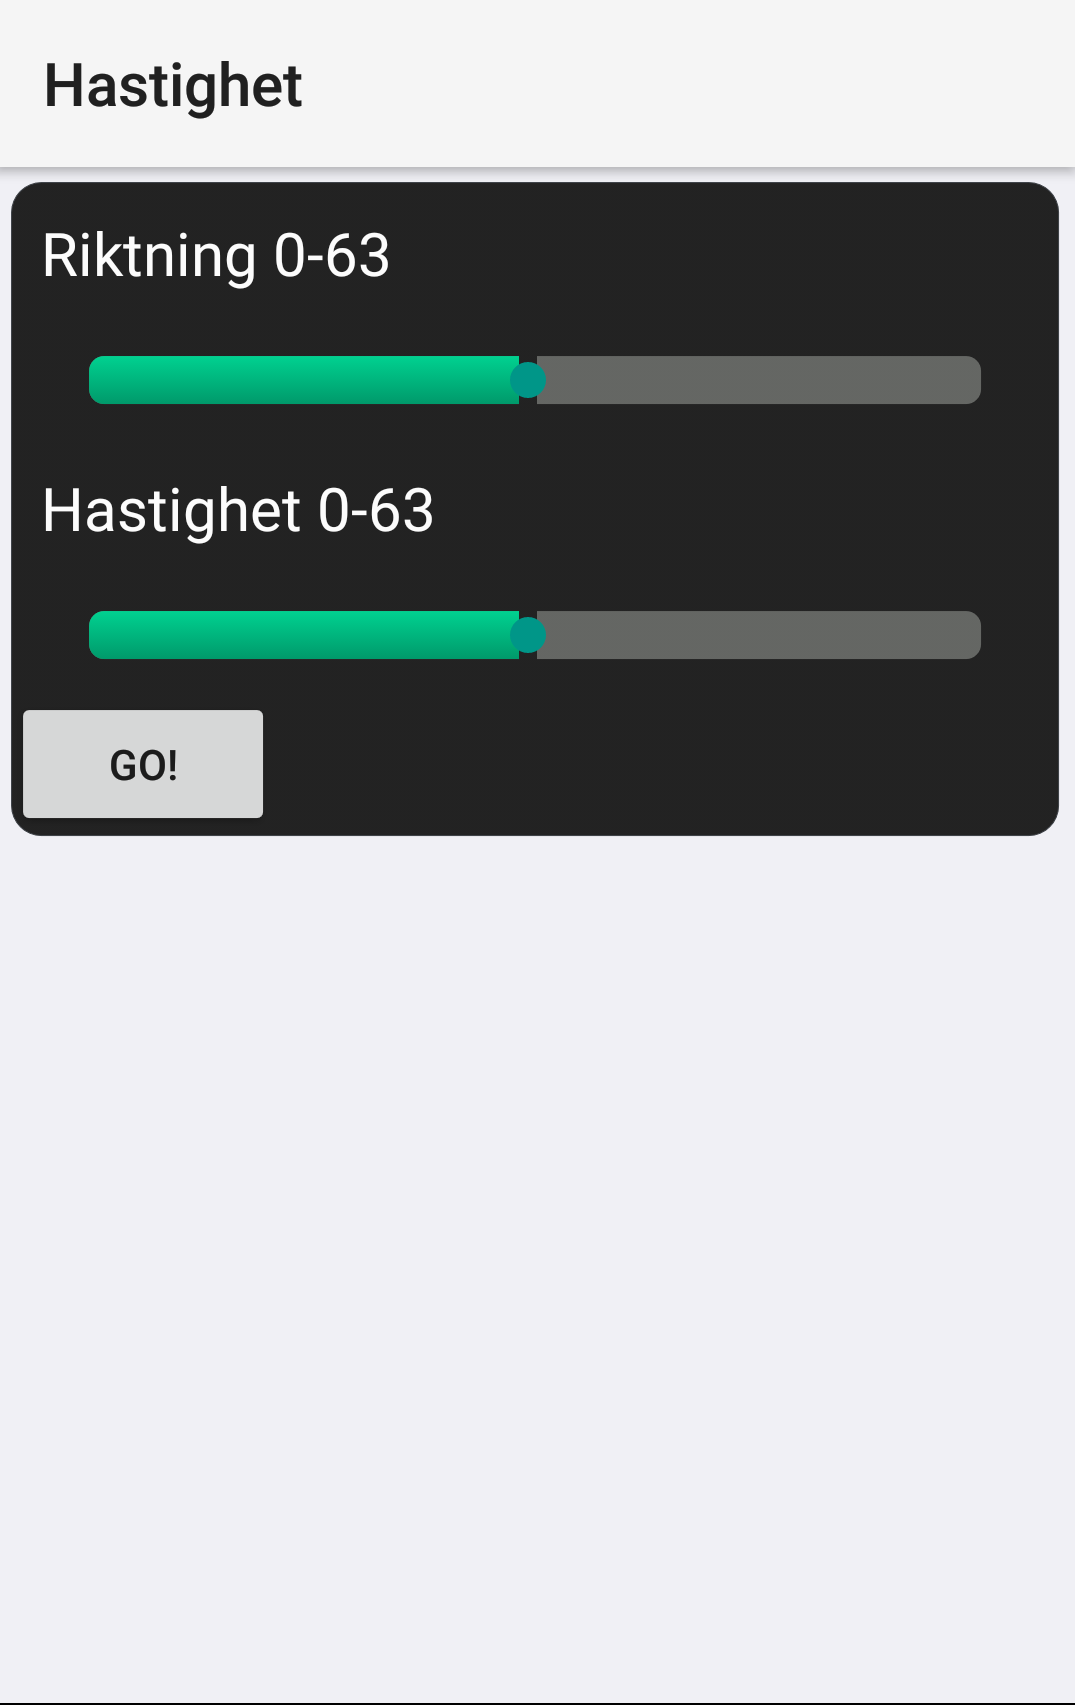
\includegraphics[scale=0.2]{Mobilapp2.png}
\centering
\caption{\it Applikationens Bluetooth-gränssnitt (vänster) samt dess virtuella reglage (höger).}
\end{figure} 

\subsubsection{Kontrollapplikation}
Kontrollapplikationen kan aktiveras från en sändande enhet. Båda sändarnoderna, MD407 samt Androidapplikationen, har möjlighet att starta denna. På MD407 görs detta genom att koppla en kabel till en specifik port, på Androidapplikationen finns istället en knapp som aktiverar denna funktion.


\vspace{5mm} \noindent
En $10\mu s$ hög puls triggar igång avståndsmätaren. Då detta sker får porten för eko på avståndsmätaren värdet 1 och ultraljud skickas ut i 8 stycken 40kHz-pulser~\cite{DistMeasure}. Om ultraljudet återvänder sätts eko-porten till 0 och pulsens bredd används för att bestämma avståndet till objektet. Detta sker genom att funktionen för kontrollapplikationen ökar en variabel inkrementellt efter varje $\mu s$. Detta tal dividerat med 58 ger avståndet till hindret i cm~\cite{DistMeasure}. Ifall inget hinder uppmäts efter en viss tid sänks pinnens värde till 0, pulsens längd tydliggör då att inget hinder finns i närheten.


\newpage
\noindent
Funktionen som styr kontrollapplikationen implementeras i mottagaren. När kommandot från sändarnoden indikerar aktivering av denna funktion skickas värdet 155 till motorn, vilket får bilen att köra i medelhög fart. Bilen fortsätter köra i denna hastigheten tills variabeln som mäter $\mu s$ uppnår värdet 8000, alternativt ungefär 138 cm. Värdet till motorn sänks då till 151, vilket motsvarar en låg fart. Denna hastighet pågår tills bilen befinner sig 1750$\mu s$ ifrån hindret, då den påbörjar motorbromsning.


\subsubsection{Radiolänk via Bluetooth}
Det som möjliggör kommunikation mellan sändare och mottagare är en Bluetooth-modul. Två likadana moduler kopplas till respektive datorenhet vilka då kan sända samt ta emot data från dessa. Modulerna är antingen konfigurerade till att vara Master eller Slave. Master-modulen letar aktivt efter en Slave-modul i närheten och kan vid upptäckt elektroniskt kopplas till den. Detta leder till att Master kan skicka data till Slave utan att riskera störningar från andra Bluetooth-enheter.


\subsubsection{MD407 som mottagarnod}
Signalerna som sändaren skickar hanteras av mottagarens datorenhet. När programmet på denna dator påbörjas måste datorn initialt skicka PWM-signaler som motsvarar neutralt läge för drivmotorn i en kort stund innan övriga signaler kan sändas. Efter detta börjar mottagaren seriellt ta emot bytes från sändaren genom sin Bluetooth-mottagare. Enheten startar även PWM-signalsgenerering till bilens styrelektronik. 

\vspace{5mm} \noindent
Varje mottagen byte analyseras i mening att skicka en PWM-signal till korrekt elektronik i bilen. Som tidigare nämnt indikerar de 2 mest signifikanta bitarna till vilken del i styrelektroniken de resterande 6 bitarnas värde ska till. De 6 minst signifikanta bitarna kommer ha ett värde mellan 0-63 när mottagaren får dem. Till detta adderas en offset på 110 vilket gör att värdet istället befinner sig i intervallet 110-173. Syftar kommandot exempelvis på motorn (se Figur 9) kommer bilen åka i högsta möjliga hastighet bakåt vid värdet 110. Farten minskar sen vid högre värden och bilen når neutralt läge vid 142. Värden över detta upp till 173 får bilen att öka farten. Detta skickas sedan som PWM-signal till bilens styrelektronik som agerar med korrekt funktionalitet. Erhåller bilens elektronik värden utanför detta intervall kan en överbelastning av bilens elektronik ske, detta märktes under projektutvecklingen då bilens styrservo förstördes på grund av detta. 



%Utöver detta kan en kontrollapplikation påbörjas(FORTSÄTT VID MER INFO). 

\begin{figure}[H]
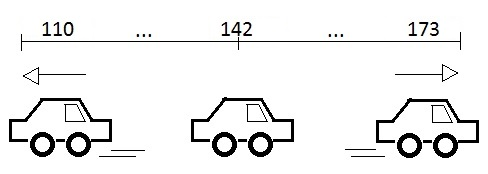
\includegraphics[scale=1]{110-173Car.jpg}
\centering
%SE ÖVER CAPTION, DENNA TEXT ÄR NÄMND I TEXTEN OVAN, ONDIG DÅ KANSKE
\caption{\it Illustrering av värdens effekter på bilen.}
\end{figure} 



%Datorn i bilen tar då emot ett kommandokod från Bluetooth-länken och analyserar detta i mening att specificera vilket kommando de två bitarna syftar på ska utföras. PWM-signalerna ändras sedan efter värdet på kommandot, de sex minst signifikanta bitarna, eller påbörjar kontrollapplikationen för demonstration. Motorerna tar emot PWM-signalerna och ger utslag beroende på deras medelspänning.

\subsubsection{Styrsignaler}
%Bilen uppfattar PWM-signaler 72 gånger i sekunden. De ursprungliga signalerna skickas på en frekvens av 72Hz, i mening att replikera dessa ges TIM2s räknare en frekvens av 100kHz. Ett antal klockcykler divideras med denna frekvens och kvoten ska då hamna nära 1/72. Antalet klockcykler är således bestämda till 1388. Resultatet av detta är att de nya PWM-signalerna skickas 72 gånger i sekunden till bilen som styrelektroniken läser av.

Bilens styrelektronik erhåller PWM-signaler från mottagaren. Under en period av klockcykler skickas delvis maximal spänning och delvis ingen spänning alls. Det antal klockcykler som skickar maximal spänning motsvarar det värde mottagaren erhållit från sändaren. Det som styrelektroniken då svarar på är hur stor andel av perioden som hög spänning mäts upp (se exempel i Figur 10). Denna procentenhet motsvarar en medelspänning som bilens styrelektronik direkt reagerar på. Intervallet som elektroniken i detta projekt svarar på är en andel på ungefär 8\%-12.4\%, alternativt en medelspänning på 269mV-423mV. Det förstnämnda värdet ger den maximala vänsterlutningen eller den högsta hastigheten bakåt beroende på vilket kommando som informationen från sändaren syftar på. Bilen kommer istället nå sin maximala högerlutning respektive högsta hastighet framåt om värdet är det sistnämnda. Intervallets mittersta värde ger ett neutralt läge i båda fallen.


\begin{figure}[H]
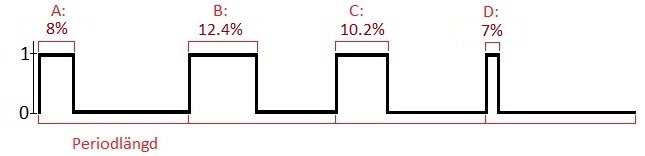
\includegraphics[scale=1]{PWMsignals.jpg}
\centering
\caption{\it Exempel på möjliga PWM-signaler. Om kommandot indikerar motorpåverkning kommer den i fall A och B köra i högsta fart baklänges respektive framlänges. I fall C hamnar bilen i neutralt läge och står då stilla.}
\end{figure} 




\newpage
\section{Resultat}
Den resulterande produkten har under projektets tid nått verifikationspunkter. Dessa beskrivs nedan i den ordning de utförts och dessutom är det förklarat om de uppnåtts eller ej. För att kunna fastställa hur bra det ersättande systemet fungerar jämförs signalerna till bilen kontinuerligt så att det hela tiden skickas identiska signaler som i det ursprungliga systemet. Efter detta anges resultatet av hur väl projektplanen följts.

%Verifikationspunkter anges nedan och resultatet beskrivs efteråt.

\subsection{MD407 som sändarnod}
Den sändande datorenheten MD407 verifieras på följande punkter:
\begin{itemize}
\item MD407 kan generera kommandosignaler.
\item Potentiometern ger rätt spänning till MD407.
\item Datorenhetens ADC ger digitala värden i korrekt intervall.
\item Kontrollapplikationen startas och utförs när detta begärs.
\end{itemize}

\noindent
Resultatet av detta är ett fullt fungerande system. MD407 kan vid testning generera signaler direkt till mottagaren. Detta fungerar även när den erhåller värden från potentiometrarna. Dessa översätts korrekt till digitala värden som sedan kan skickas från sändarnoden. Dessutom kan kontrollapplikationen aktiveras och utföras på rätt sätt.


\subsection{Androidapplikation som sändarnod}
Följande punkter har verifierat att Androidapplikationen fungerar enligt specifikation:

\begin{itemize}
\item Det är möjligt att aktivera telefonens Bluetooth och upprätta en anslutning till bilens Bluetooth-modul.
\item Adroidapplikationen kan skicka värden till den mottagande enheten som ger korrekt följd.
\item Kontrollapplikationen startas och utförs när detta begärs.
\end{itemize}

\noindent
Applikationen fungerar som förväntat. Den kan aktivera Bluetooth och på så sätt ansluta till mottagarens modul. Emellertid kopplar telefonens inbyggda Bluetooth betydligt snabbare till mottagarens än de tilläggsfunktioner som funnits tillgängliga till applikationen. Rätt värden skickas och bilens agerande efter detta är korrekt. Även kontrollapplikationen aktiveras och utförs riktigt.

\newpage
\subsection{Kommunikationslänk}
Informationsflödet mellan datorenheterna har testats i tre nivåer kontinuerligt under projektets gång:
\begin{itemize}
\item Kommunikation är möjligt via direktkopplad kabel.
\item Information kan sändas och mottas via RF-moduler.
\item Sändaren kan skicka information till mottagaren via Bluetooth.
\end{itemize}

\noindent
Vid slutfört projekt kunde alla punkter uppfyllas. Bilens ersättande mottagare har kunnat kommunicera med sändaren via en direktkopplad kabel, en RF-modul och till slut en Bluetooth-modul. När något ej fungerat i flödet mellan sändare och respons på styrsignal har kommunikationen förflyttats till den första nivån för att förenkla felsökning.

\subsection{MD407 som mottagarnod}
En mottagande MD407 har verifierats enligt följande punkter:

\begin{itemize}
\item Skickar rätt PWM-signal till styrelektronik.
\item Kan ta emot värden från sändande enhet.
\item Har den ursprungliga bilens funktionaliteter.
\item Kan initiera kontrollapplikationen efter aktivering från en sändarnod.
\end{itemize}

\noindent
Resultatet är ett fungerande system. Värden tas emot via en inkopplad Bluetooth-modul. Enligt oscilloskop bekräftas värdena till bilens styrelektronik vara identiska. Samtliga funktioner i det ersättande systemet har testats och fungerar som ursprungligen. Det vill säga hastigheten framåt och bakåt samt rattutslagen åt vänster och höger har verifierats vara korrekta. Mottagaren startar dessutom kontrollapplikationen och utför denna på rätt sätt efter aktivering från en utav sändarnoderna.




\subsection{Kontrollapplikation}
Nedanstående punkter användes för att testa kontrollapplikationen.

\begin{itemize}
\item Stannar enligt specifikationer maximalt 1 cm från ett hinder vid maximala hastighet.
\item Fungerar från sändande MD407.
\item Fungerar från sändande Androidapplikation.
\end{itemize}

%Rättstavningen klagar på förbestämts men det är väl rätt?

\noindent
Verifieringspunkterna har till viss del uppnåtts. Implementation av aktivering från båda sändarnoderna fungerar korrekt. Kontrollapplikationen är funktionell på en maximal hastighet som förbestämts utifrån att inte riskera att få opålitlig data från avståndsmätaren. Däremot stannar bilen inte på det angivna avståndet, utan har en större marginal.


\subsection{Verifikation av projektplan}
Mindre förändringar har under projektets gång skett men i övrigt har projektplanen följts. Då ersättandet av kontrollen samt bilens  mottagare varit mer komplicerad än projektgruppen trott tog denna procedur 3 veckor längre än väntat. Detta problem har troligtvis försämrat kvalitén på kontrollapplikationen men ej Androidapplikationen då denna konstruerats parallellt med den nya sändar- samt mottagarnoden. Utöver detta har versionshanteringssystemet möjliggjort för enkel fildelning och Slack har varit fördelaktigt vid distribuerande av information. Veckomötena gav en bra överblick över hur det gått för de olika arbetslagen och problem som uppkommit under veckan kunde där lösas.



\newpage
\section{Diskussion och Slutsats}
%TA MED ATT DET TOG LÄNGRE TID BC FEL I BIBLIOTEK, STYRSERVO SÖNDER

%VARFÖR MÅL 1 TOG LÄNGRE TID
Projektet följde ej tidsmodellen som givits i planen. Ett antal fel i de tillhandahållna biblioteken ledde till extra verifikation för att kunna erhålla rätt hjälpfunktioner. Utöver detta slutade bilens styrservo att fungera på grund av att felaktiga PWM-signaler skickats till styrelektroniken som då överbelastades. Dessutom var implementationen av de ersättande mottagar- och sändarnoderna mer invecklade än vad som uppfattats vid början av projektet och detta krävde därför mer tid än vad som gavs i projektplanen. Parallellt arbete utnyttjades dock, vilket mildrade effekten av uppgiften som tagit mer tid än beräknat. 

%HANDKONTROLL
\vspace{5mm} \noindent
Projektgruppen vill belysa en vidareutveckling av sändar- samt mottagarnod. Delsystemen är endast hårdvarunära implementerade, ett konsumentvänligt lager finns ej. Detta möjliggör för stor frihet i designen för en butiksfärdig produkt. Ett användarvänligt skal skulle kunna konstrueras för både den ersättande handkontrollen och bilen med den nya mottagaren. 


%ANDROIDAPPLIKATION
\vspace{5mm} \noindent
Med Androidapplikationen ses stora möjligheter. 2013 ägdes en smartphone av ungefär 90\% av Sveriges befolkning mellan 12-45 år~\cite{smartphoneStat}. Telefonapplikationen vänder sig till en väldigt stor andel av folket och projektgruppen ser därför positivt på att utveckla denna. Fokuset med Androidapplikationen har varit på en hårdvarunära nivå och utseendet är därför inte så tilltalande. Ur ett designperspektiv är till exempel inte de två reglage som applikationen använder sig av optimala för styrning av bilen. En bättre lösning hade varit att ersätta reglagen med en joystick. Applikationen skulle även kunna bli mer användarvänlig genom att implementera taktil återkoppling, exempelvis via vibrationer. På lämpligt sätt kan även en sammanställning av skärmen för styrning och Bluetooth-gränssnitt hjälpa Androidapplikationen. Utöver detta skulle applikationen kunna implementeras på ett flertal operativsystem och således vara tillgänglig för en större mängd användare. 

\vspace{5mm} \noindent
Androidapplikationen skulle kunna användas till flera olika ändamål. Förutom att den är praktisk då den externa handkontrollen inte längre behövs skulle en användare kunna ansluta till ett flertal bilar via sin applikation. Denna användare skulle då kunna styra andra radiobilar så länge de har en mottagande Bluetooth-modul och likadana kommandofunktioner. Detta skulle vara användbart då risken för att bilens handkontroll kommer bort eller förstörs elimineras. Även kostnaderna för produkten minskas både för tillverkare och konsument eftersom handkontrollen inte behövs. Skulle denna styrning möjliggöras kan det dock behövas att konstruera ett säkerhetslager så att oinbjudna parter ej kan ta kontroll över bilen.



%HUR VI BESTÄMDE SPECIFIKATIONER ÖVER KONTROLLAPPLIKATION
\newpage
\noindent
Kontrollapplikationen kunde ej färdigställas efter givna mål. Enligt specifikationen skulle bilen stanna högst 1 cm från närmaste hinder, men detta kunde ej uppnås med den ålagda tiden för uppgiften. Det finns flera felkällor som bidragit till svårigheter i utvecklingen. För det första har avståndsmätaren varit mer opålitlig än förväntat vilket lett till att inkonsekventa värden tagits emot. För det andra är bilens egna bromssystem svagt och påverkas av batteriets styrka. Det är därmed svårt att förutsäga bromssträckan. För det tredje störs avståndsmätaren av vibrationer från bilens motor vilket försämrar noggrannheten av uppmätningen ytterligare. 

\vspace{5mm} \noindent
Ett par faktorer hade kunnat förbättra kontrollapplikationen. En avläsningsalgoritm som bättre filtrerar värden hade givit mer fördelaktig data som noggrannare kunnat beräkna tiden då bilen ska påbörja motorbromsning. Dessutom hade en funktion som mäter bilens hastighet kunnat användas till att bestämma rätt inbromsningsavstånd beroende på farten. Dessa faktorer hade kunnat resultera i en bättre kontrollapplikation som möjliggjort för större kontroll över bilen.



\vspace{5mm} \noindent
Sammanfattningsvis innehåller detta projekt en radiostyrd bil med modern teknik. Uppgradering med nya datorer reducerar utdaterad teknik och dess funktioner passar väl in med det som är aktuellt idag. Grunden för systemet är utfört och stora designmöjligheter finns hos sändarnoderna samt hos mottagarnoden. Kort sagt resulterar detta projekt i en stor uppdatering till den klassiska radiostyrda bilen där modern teknik är implementerad.




\newpage
%To references
\addcontentsline{toc}{section}{Bibliografi}
\bibliographystyle{IEEEtran}
\bibliography{referenserRapport}


\end{document}

